\documentclass{beamer}
\usepackage[utf8]{inputenc}
\usepackage[russian]{babel}

\usepackage{graphicx}

\usecolortheme{orchid}

\setbeamertemplate{footline}[frame number]
\beamertemplatenavigationsymbolsempty

\title{Синтаксический анализ исходного кода, содержащего инструкции препроцессора}
\author{Савенко Сергей Андреевич}
\institute{{\tiny научный руководитель} \\ \vspace{.10cm} Игнатов Сергей Сергеевич}
\date{\scriptsize Академический университет\\ \vspace{.10cm} 2014 г.}

\begin{document}

\frame{\titlepage}

\frame{
  \frametitle{Пример непрепроцессированного кода}

  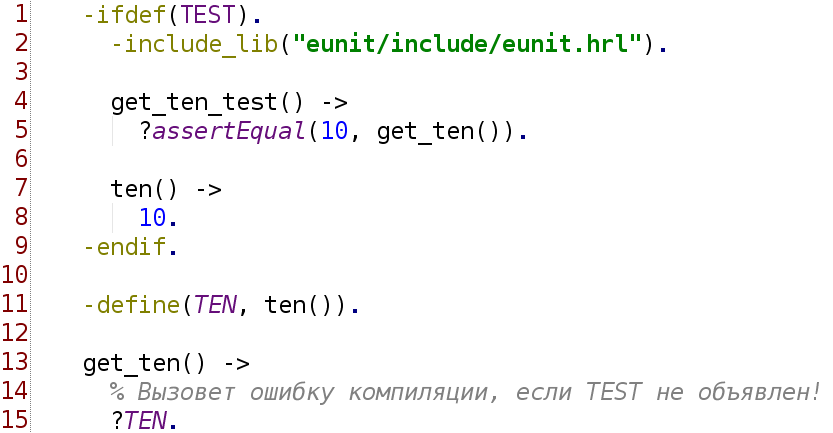
\includegraphics[width=\linewidth]{preprocessor.png}
}

\frame{
  \frametitle{Цели и задачи}

  \begin{block}{Цель работы}
    Создать инструмент, позволяющий производить синтаксический анализ исходного кода, содержащего инструкции препроцессора, используя грамматику языка программирования и интерпретатор инструкций препроцессора
  \end{block}

  \begin{block}{Задачи работы}
    \begin{enumerate}
      \item Изучить существующие решения
      \item Разработать и реализовать алгоритм синтаксического анализа непрепроцессированного кода
      \item Сравнить разработанную библиотеку с аналогами
    \end{enumerate}
  \end{block}
}

\frame{
  \frametitle{Существующие решения}

  \begin{block}{SuperC}
    \begin{itemize}
      \item LR-анализатор
      \item Парсер-генератор Bison
    \end{itemize}
  \end{block}

  \begin{block}{TypeChef}
    \begin{itemize}
      \item LL-анализатор
      \item Библиотека парсер-комбинаторов
    \end{itemize}
  \end{block}
}

\frame{
  \frametitle{Подход к разбору непрепроцессированного кода}

  Синтаксический анализ проводится в 2 этапа:
  
  \begin{block}{Частичное препроцессирование}
    \begin{itemize}
      \item Интерпретация инструкций препроцессора
      \item Сохранение информации об условных ветвлениях
      \item Результат: направленный ориентированный граф последовательностей лексем для всех ветвей условной компиляции
    \end{itemize}
  \end{block}
  
  \begin{block}{Синтаксический анализ графа лексем}
    \begin{itemize}
      \item Обработка ветвей условной компиляции
      \item Результат: синтаксическое дерево, содержащее узлы условного ветвления
    \end{itemize}
  \end{block}
}

\frame{
  \frametitle{Модифицированный алгоритм Earley}

  Алгоритм строит новое состояние для каждого входного символа --- множество элементов Earley:

  \begin{block}{Элемент Earley}
    \begin{itemize}
      \item $A \to A \beta \bullet B$
      \item Номер состояния, где был добавлен $A \to \bullet A \beta B$
      \item С каждым элементом ассоциируется множество пар [элемент-предшественник, условие наличия].
    \end{itemize}
  \end{block}

  Каждая ветвь условной компиляции обрабатывается отдельно. 
  
  Последние состояния для каждой из ветвей условной компиляции объединяются.
}

\frame{
  \frametitle{Сравнение с TypeChef}
 
  Сравнение проводилось на подмножестве языка Erlang 

  \begin{block}{Отличия разработанного решения}
    \begin{itemize}
      \item Отсутствие необходимости модификации грамматики языка
      \item Отсутствие необходимости описания ветвлений и слияний
      \item Лаконичность синтаксиса описания языка: $\sim$100 строк на Java против $\sim$200 строк на Scala
      \item Медианное время работы на тестовых данных в $\sim$2 раза меньше
    \end{itemize}
  \end{block}
}


\frame{
  \frametitle{Результаты}
  
  Разработан инструмент для создания синтаксических анализаторов исходного кода, содержащего инструкции препроцессора

  \begin{block}{Особенности решения}
    \begin{itemize}
      \item Описание грамматики языка в БНФ
      \item Автоматическое ветвление и слияние ветвей разбора
      \item Поддержка языков, порождаемых контекстно-свободными грамматиками
      \item Сравнимая с аналогами производительность
    \end{itemize}
  \end{block} 
}

\end{document}
